\chapter{The LHC and The CMS Experiment}

\section{The LHC}
The Large Hadron Collider(LHC) is the largest and most powerful superconducting hadron accelerator and collider. The LHC was installed in an existing 26.7 km tunnel that was constructed for LEP machine between 1984 and 1989. The tunnel of LHC has 8 straight sections and 8 arcs, and locates between 45m and 170m below the surface. The LHC host 4 experiments currently: CMS(Point 5), ATLAS(Point 1), ALICE(Point 2) and LCHb(Point 8).
\subsection{LHC: Performance and Main machine layout}

\begin{figure}[htbp]
 \begin{center}
  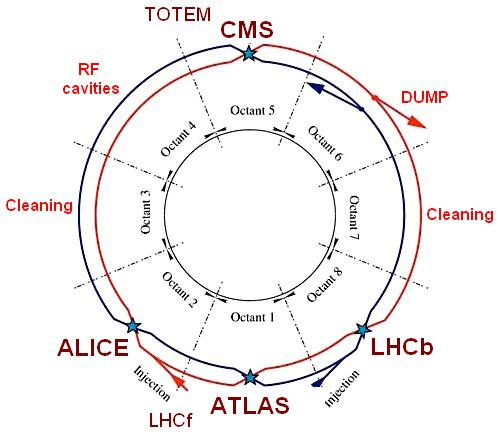
\includegraphics[width=0.8\textwidth]{figures/c3/c3_lhc_latticelayout.jpg}
 \end{center}
 \caption{abcf}
 \label{fig:c3lhclayout}
\end{figure}
Performance, eq, lumi, xsection. Lumi equation from lhc parameter.
Main machine layout: 2 beam with 2 rings, 8 long straight sections and 8 arcs.

\begin{equation}
 L = \frac{N^{2}_{b}n_{b}f_{rev}\gamma_{r}}{4\pi \varepsilon_{n}\beta *}F \;
 \label{eq:c3lhclumi}
\end{equation}

\begin{equation}
 F = (1+\frac{\theta_{c}\sigma_{c}}{2\sigma *})^{-1/2} \;
 \label{eq:c3lhcgeof}
\end{equation}

\subsection{LHC: From operation point of view}
The LHC is a extremely complex machine and it is almost impossible to grasp all details. However, the LHC is provide a summary of status for the operational activities, which are very useful in the detector operation.
\subsubsection{Acclerator Mode}
The accelerator mode provides a summary status of the LHC machine.The detector system(eg. CMS) need to make daily operational decision accroding to the accelerator mode.
\begin{table}[htbp]
\fontsize{10 pt}{1.2 em}
\selectfont
\begin{centering}
\caption{\label{tab:c3lhcaccmode} Acclerator Mode}
\hspace*{-4ex}
\begin{tabular}{|c|c|c|}
\hline
 Mode Name &  Description & Beam exist \\
\hline
 SHUTDOWN & \specialcell{Machine not running} & NO BEAM \\
\hline
 COOLDOWN & \specialcell{Machine comes back from shutdown,\\ cryogenics related activities going on} & NO BEAM \\
\hline
 MACHINE CHECKOUT & \specialcell{Checking out LHC subsystems} & NO BEAM \\
\hline
 ACCESS & \specialcell{Access going on} & NO BEAM \\
\hline
 MACHINE TEST & \specialcell{Operation tests without beam} & NO BEAM \\
\hline
 CALIBRATION & \specialcell{Power converter calibration} & NO BEAM \\
\hline
 WARM-UP & \specialcell{Sectors warm up for repair} & NO BEAM \\
\hline
 RECOVERY & \specialcell{Quench recovery} & NO BEAM \\
\hline
 SECTOR DEPENDENT & \specialcell{Sector activities going on} & NO BEAM \\
\hline
 BEAM SETUP & \specialcell{Machine setup with 1 or 2 beams,\\ usually a signal of next physics fill when taking data} & BEAM \\
\hline
 PROTON PHYSICS & \specialcell{Beam on for proton physics} & BEAM \\
\hline
 ION PHYSICS & \specialcell{Beam on for ion physics} & BEAM \\
\hline
 TOTEM PHYSICS & \specialcell{Beam on for TOTEM physics} & BEAM \\
\hline
 MACHINE DEVELOPMETN & \specialcell{Beam on machine development} & BEAM \\
\hline
\end{tabular}
\par\end{centering}
\end{table}

\subsubsection{Beam Mode}

\begin{table}[htbp]
\fontsize{10 pt}{1.2 em}
\selectfont
\begin{centering}
\caption{\label{tab:c3lhcbeammode} Beam Mode}
\hspace*{-4ex}
\begin{tabular}{|c|c|c|}
\hline
 Mode Name &  Description \\
\hline
 SETUP & \specialcell{Beam in transferline, but not in the ring} \\
\hline
 ABORT & \specialcell{Recovery mode following bram drop} \\
\hline
 INJECTION PROBE BEAM & \specialcell{Ring is injected with test beam for safe circulating} \\
\hline
 INJECTION SETUP BEAM & \specialcell{Beam measurement going on after probe beam\\ but before injection physics beam} \\
\hline
 INJECTION PHYSICS BEAM & \specialcell{Beam for physics is injected in the ring} \\
\hline
 PRERAMP & \specialcell{Injection done, prepare for ramp} \\
\hline
 RAMP & \specialcell{Ramp up the beam energy} \\
\hline
 FLAT TOP & \specialcell{Ramp done, pre-squeeze checks} \\
\hline
 SQUEEZE & \specialcell{Squeezing the beam size} \\
\hline
 ADJUST & \specialcell{Preparing for collision after collision} \\
\hline
 STABLE BEAMS & \specialcell{Stable collision, detector should taking data} \\
\hline
 UNSTABLE BEAMS & \specialcell{Unstable beam because of sudden beam degradation} \\
\hline
 BEAM DUMP WARNING & \specialcell{Beam dump warning in case of emergency beam dump} \\
\hline
 BEAM DUMP & \specialcell{End of physics collision} \\
\hline
 RAMP DOWN & \specialcell{Ramp down beam energy after programmed dump} \\
\hline
 CYCLING & \specialcell{Pre-cycle before injection\\ following access, recovery, etc} \\
\hline
 NO BEAM  & \specialcell{No beam exist} \\
\hline
\end{tabular}
\par\end{centering}
\end{table}

\subsubsection{Operation Mode}

\section{The CMS Experiment}

The CMS Experiment is a particle physics experiment based on CMS detector system on the LHC. It contains with CMS detector system and event reconstruction, supported by the detector operation team, computing/storage department and software fraction.

\subsection{CMS Detector System}

The Compact Muon Solenoid (CMS) is one of the general-purpose detection system on the LHC. To fullfill the "general-purpose", the CMS is designed as a combo of several subsystems: Sillicon Pixels and Strips for tracking information, Electromagnetic and Hadron Calorimeters for "light" particle energy deposition and drift tubes and cathode strip/resisstive plate chambers for muon details. The locations of these subdectors in the CMS are not random: The sillicon tracking subsystems are located on the inner CMS, closest to the collision point, and the calorimeter subsystems after the sillicon subdetectors, because of its destructive detection nature; Finally the muon system in the outer layer to capture our heavy object which go through the calorimeter subsystems. To obtain the high performance, the CMS is immersed in a 4-T field, which is powered by a superconducting solenoid("S" in CMS). The magnet components have a major contribution on the CMS total weight: 12500 tones out of 14000. However, comparing with its heavy weight, the size of the CMC system is relatively small: only 5000 $m^{3}$. Then the given name "Compact" is imposed in front of "Muon Solenoid" since its density near to 3000 $kg/m^{3}$.

\subsubsection{Inner Tracking system}

As described in the name - - - inner tracking system, there are two main features for this CMS sub-detector: the closest sub-detector to the LHC beam and tracks reconstruction. The main challenge is a consequence of the first feature: the inner tracking systems have to be radiation hard during the expected lifetime of 10 years (LHC run1+run2+run3). More over, since the LHC have high intensity and small bunch crossing (25ns), we also need the inner tracking systems to have a fine granularity and fast response. The silicon based technology detector is the best option to satisfy all these requirements. On the other hand, the second feature actually comes from the physics requirement. We need to reconstruct the tracks of charged particles and secondary vertices in the event from the three dimensional hits. The tracks information are not only used in the charged particle reconstruction, but also applied in the particle flow algorithm as a base of all physics objects in CMS collaboration. The secondary vertices are also important in the heavy flavor objects reconstruction, and new physics search of long-lived particles. 

As a result of budget-performance balance, the CMS inner tracking systems are designed as a combination of two sub-systems: the silicon pixel and the silicon strip. A schematic drawing of the CMS tracking system is shown in the Fig.~\ref{fig:c3cms2dtracker}. More details will be described in the following sections. 

\begin{figure}[htbp]
 \begin{center}
  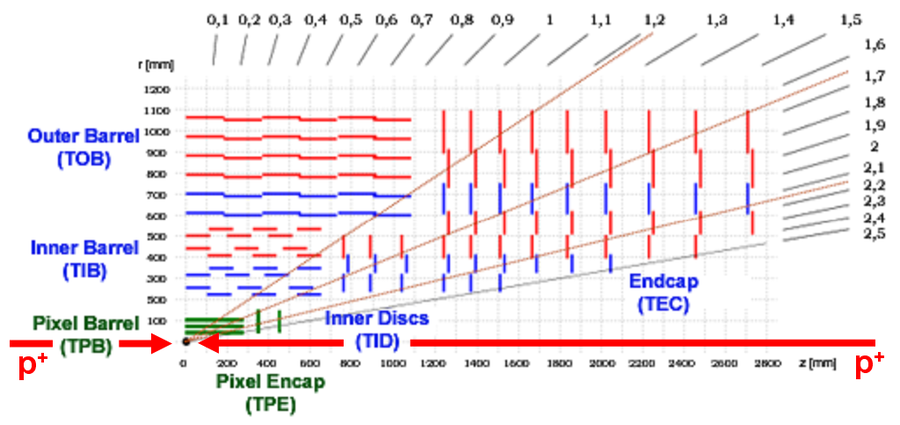
\includegraphics[width=0.8\textwidth]{figures/c3/c3_cms_2dtracker.png}
 \end{center}
 \caption{Two dimensional CMS inner tracking system layout, phrase 0}
 \label{fig:c3cms2dtracker}
\end{figure}

\paragraph{Silicon Pixels}

The pixel system is the part of inner tracking system that closest to the collision point. It provides a precise measurement of the tracking points; therefore contribute a lot for the secondary vertex reconstruction. The pixel cells are distributed with size of 100 num*150 num in three-dimensional space, which allow a 3D reconstruction method for the secondary vertex offline. Readout chips bump bonded to the sensor read out the signals from pixel cells. Then the signal will be delivered to the frondend driver through the analog chain once we receive a positive bit from L1 trigger.

The phrase 0 pixel detector contains three barrel layers (BPix) and two endcap disks (FPix), which covers a pseudo rapidity range $-2.5<\eta<2.5$. In phrase 1 upgrade, to suffer from the radiation damage, we replaced all layers and disks with new ones, and added one layer in the barrel region, one disk in the endcap region.

One special design of the pixel detector is the blade that module mounted are rotated by 20 degrees in a turbine geometry. Such an arrangement enhanced the charge sharing effects between the nearby pixels. The space resolution can be improved to 15num by the using the “charge sharing” effect in pixels. CMS take advantage of this effect with the analog readout of the collected charges by readout pixels in-group with readout chips. 

\paragraph{Silicon Strips}

The particles pass through ten layers of silicon strip detectors after the pixel. The strip detector provides a complete charged track together with the pixel detector. The silicon strip tracker is composed of 15148 detector modules. Each module carries either one 320 num or two 500 num silicon sensors from a total of 24244 sensors. The charges that come out of sensor will be amplified, shaped and stored by a custom integrated circuit. Once received a positive L1 trigger decision, the analog signal will be multiplexed and transmitted via optical link to the front end driver, then digitalized. 

The inner strip detector contains 4 barrel layers (TIB) and 3 disks (TID) support for each side. The outer strip detector has 6 barrel layers (TOB, 2 double-sided, 4 single-sided) and the endcap strip has 9 disks (TEC) on each side.

The online alignment system for the strip detector is necessary with the complicate structure and resolution requirement in physics performance. The laser alignment system is designed and built in to monitor the stability and the alignment of the strip detector mechanical structure. The infrared laser light will be delivered directly to the sensor on the 434 silicon modules (3\%) to trigger a signal pulse. The alignment data can be taken during commission, inter-fill period and also in the orbit gap when we have stable beam. Since the pixel will be aligned with strip through the reconstructed tracks, the strip alignment is the only online and direct alignment for the whole inner tracking system. 


\subsubsection{Calorimeters}
\paragraph{Electromagnetic Calorimeter}
\paragraph{Hadron Calorimeter}

\subsubsection{Muon Detectors}

The importance of the Muon detectors is implied by the experiment’s middle name (“M” is CMS). The CMS muon detectors provide precise measurement of muon tracks with the support of strong magnet field (3.8T). The measurement of muons is useful in both standard model physics (e.g. Higgs to ZZ) and new physics search (e.g. leptonic channel supersymmetry). More over, the muon system also provide muon related trigger to reduce the data rate.

The CMS muon detectors consist of three sub-detectors: Drift tube in the barrel region, cathode strip chamber in the endcap and resistive plate chamber in both barrel and endcap. A layout of CMS muon detectors are showed in the Fig.~\ref{fig:c3cms2dmuondets}. More details are demonstrated in the following sections. 

\begin{figure}[htbp]
 \begin{center}
  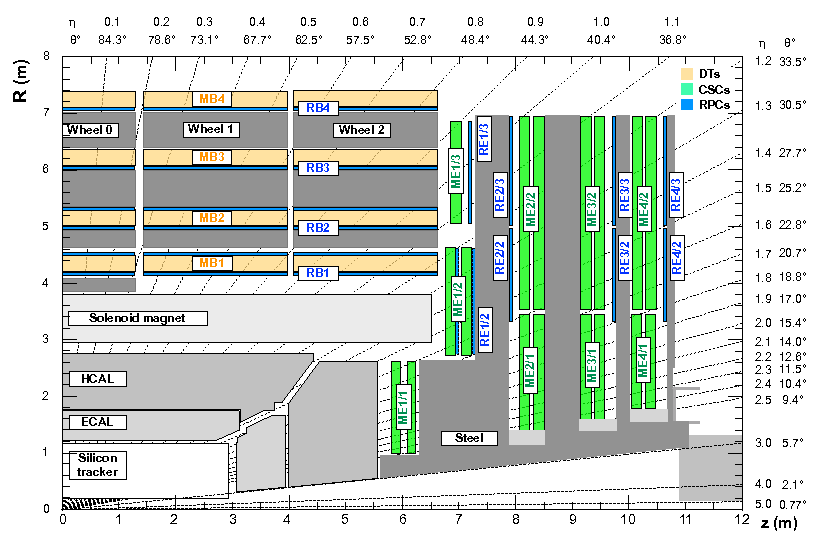
\includegraphics[width=0.8\textwidth]{figures/c3/c3_cms_2dmuondets.png}
 \end{center}
 \caption{Two dimensional CMS inner tracking system layout, phrase 0}
 \label{fig:c3cms2dmuondets}
\end{figure}

\paragraph{Drift Tubes}
Drift tubes (DT) are the part of CMS muon detectors that measure the muon tracks in the barrel region. The basic unit of the drift tubes is the drift cell. A drift cell is a 42mm-wide tube contains a thin conductive wire at high positive voltage within a gas volume. The muon knocks electron off the atom of the gas when it travel through the tube. The muon tracks can be reconstructed by measuring the drift time for different cells. 

Like the HCAL outer, the Drift tubes contain 5 wheels along the z-axis, 4 stations for each wheel, labeled as MB1, MB2, MB3 and MB4. The three inner stations have 60 drift chambers each and the outer chamber has 70. A drift chamber consists of 2 or 3 super layers, each made of by 4 layers of drift cells staggered by half of cell. This honeycomb geometry gives an excellent time-tagging capability, with a time resolution of a few nanoseconds. The full DT provides the pseudo-rapidity coverage $0<|\eta|<1.2$.

\paragraph{Cathode Strip Chambers}
Cathode strip chamber (CSC) is one of the CMS muon detectors that located in the endcap region. CSC is also a type of wire chamber, but different from the DT, CSC measures the location (to be specific, phi coordinates) instead of drift time. The CSC consists arrays of positively charged anode wires crossed with negatively charged copper cathode strip within a gas volume. The muon will knock the electron off from the gas atom. Then the electron will move to the anode wire to create an avalanche. Positive ions also move to the cathode and trigger a charged pulse.

The CMS endcap muon system consists of 468 cathode strip chambers in the following arrangement: 72 ME1/1, 72 ME1/2, 72 ME1/3, 36 ME2/1, 72 ME2/2, 36 ME3/1, 72 ME3/2, and 36 ME4/1. The full CSC provides the pseudo-rapidity coverage $1.2<|\eta|<2.4$. 

As we will mention at the beginning of next section, the RPC is designed as a fast response provider to trigger. However, for the endcap region, CSC is already good enough to satisfy the trigger requirement in the current instantaneous luminosity of the LHC. Moreover, CSC has a better spatial resolution and more pseudo-rapidity coverage, which provide a precise measurement for the endcap muons.

\paragraph{Resistive Plate Chambers}
Resistive plate chamber (RPC) is a fast gaseous detector that provides a muon trigger system in parallel with the DT and CSC. The RPC is a two high resistively plastic parallel plates system with gas in the middle. One of the plates is the positively charged anode and the other is negatively charged cathode. Like the CSC, the electron of gas will be knocked off when muon pass through, and then trigger avalanche. The pattern of hits on the cathodes will provide a quick measurement on the muon momentum and then pass to trigger for decision-making. In the CMS RPC, we are using the double-gap module instead of the single-gap one. This allows a lower bias voltage requirement of each single-gap and higher detector efficiency. The RPC performance is a combination of good spatial resolution and time resolution (one nanosecond). 

The CMS RPCs are distributed in both barrel and endcap region. There are 96 RPCs each wheel in barrel region. More details of the distribution are listed in the Table~\ref{tab:c3cmsrpc}. In the endcap region, we have 3 RPC stations in the phrase 0 design. In order to keep the high muon reconstruction efficiency with run2 condition, the fourth disk is installed during the long shutdown 1 for the phrase 1 upgrade. The full RPC have the same pseudo-rapidity coverage as DT in barrel, and smaller coverage ($1.2<|\eta|<2.1$) than CSC in endcap.

\begin{table}[htbp]
\fontsize{10 pt}{1.2 em}
\selectfont
\begin{centering}
\caption{\label{tab:c3cmsrpc} Numbers of RPCs for different wheels}
\hspace*{-4ex}
\begin{tabular}{|c|c|c|c|c|c|c|}
\hline
 RPC &  W+2 & W+1 & W0 & W-1 & W-2 & Total \\
\hline
 RB1(in) & 12 & 12 & 12 & 12 & 12 & 60 \\
\hline
 RB1(out) & 12 & 12 & 12 & 12 & 12 & 60 \\
\hline
 RB2/2(in) & 12 & - & - & - & 12 & 24 \\
\hline
 RB2/2(out) & - & 12 & 12 & 12 & - & 36 \\
\hline
 RB2/3(in) & - & 12 & 12 & 12 & - & 36 \\
\hline
 RB2/3(out) & 12 & - & - & - & 12 & 24 \\
\hline
 RB3 & 24 & 24 & 24 & 24 & 24 & 120 \\
\hline
 RB4 & 24 & 24 & 24 & 24 & 24 & 120 \\
\hline
 Total & 96 & 96 & 96 & 96 & 96 & 480 \\
\hline
\end{tabular}
\par\end{centering}
\end{table}


\subsubsection{Trigger system}


\subsection{Event Reconstrunction}
\subsubsection{Particle Flow}
\subsubsection{Tracks}
\subsubsection{Electrons}
\subsubsection{Muons}
\subsubsection{Jets and Missing Transverse Energy}
